\documentclass{beamer}
\usetheme{Madrid}
\usecolortheme{default}
\usepackage{listings}
\usepackage{tcolorbox}
\tcbuselibrary{listings, skins}

\newtcblisting{mycode}{
  arc=0mm,                          % Sharp corners
  boxrule=0.5pt,                    % Border thickness
  colback=white,                    % Background color
  colframe=black,                   % Border color
  listing only, 
  listing options={
    language=Python,
    basicstyle=\small\ttfamily,      % Monospace font
    keywordstyle=\color{blue},       % Color for 'import', etc.
    commentstyle=\color{blue},       % Color for comments
    stringstyle=\color{red},
    showstringspaces=false,
    breaklines=true
  },
  sharp corners,
  enhanced,
}

\title{Analog-1.1.27}
\author{INDHIRESH S-EE25BTECH11027}
\date{\today}

\begin{document}

\begin{frame}
    \titlepage
\end{frame}

\begin{frame}{Question}
Consider the op-amp circuit shown.
\begin{figure}[H]
    \centering
    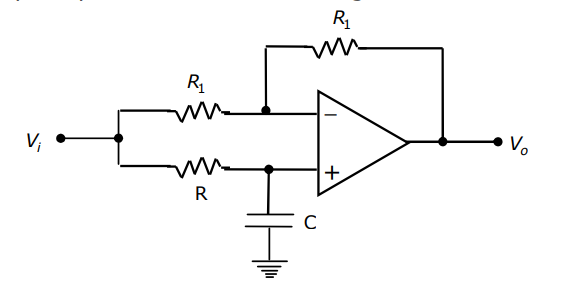
\includegraphics[width=0.4\linewidth]{ques.png}
    \caption{Op-amp circuit}
    \label{fig:placeholder}
\end{figure}
\begin{enumerate}

\item The transfer function Vo(s)/Vi(s) is:\\

\begin{columns}[t]
    \column{0.2\textwidth}
    1) $\frac{1-sRC}{1+sRC}$
    \column{0.2\textwidth}
    2) $\frac{1+sRC}{1-sRC}$
    \column{0.2\textwidth}
    3) $\frac{1}{1-sRC}$
    \column{0.2\textwidth}
    4) $\frac{1}{1+sRC}$
\end{columns}
\vspace{20pt}
\item If Vi = Vi sin($\omega$t) and Vo = Vo sin($\omega$t + $\phi$), the minimum and maximum values of $\phi$ (in radians) are respectively:
\begin{columns}[t]
    \column{0.2\textwidth}
    1)-$\frac{\pi}{2}$ and $\frac{\pi}{2}$
    \column{0.2\textwidth}
    2)0 and $\frac{\pi}{2}$
    \column{0.2\textwidth}
    3) -$\pi$ and 0
    \column{0.2\textwidth}
    4)-$\frac{\pi}{2}$ and 0
\end{columns}
\end{enumerate}
\end{frame}


\begin{frame}{PART-A: Ideal Assumptions}
    For an ideal operational amplifier analysis:
    \vfill
    \begin{itemize}
        \item \textbf{Infinite Input Impedance:} No current enters the terminals ($I_+ = I_- = 0$).
        \item \textbf{Infinite Open-Loop Gain:} Forces a \textbf{Virtual Short} between inputs:
        \begin{equation*}
            V_+ = V_-
        \end{equation*}
        \item \textbf{Zero Output Impedance:} The output can drive any load without voltage drop.
    \end{itemize}
\end{frame}

\begin{frame}{Analysis of the Non-Inverting Node ($V_+$)}
    The input $V_i(s)$ passes through a series $RC$ network to ground. Using the \textbf{Voltage Divider Rule}:
    \begin{equation}
        V_+(s) = V_i(s) \cdot \frac{\frac{1}{sC}}{R + \frac{1}{sC}}
    \end{equation}
    \vfill
    Multiply numerator and denominator by $sC$:
    \begin{equation}
        V_+(s) = \frac{1}{1 + sRC} V_i(s)
    \end{equation}
\end{frame}

\begin{frame}{ Analysis of the Inverting Node ($V_-$)}
    Applying KCL at the inverting node (assuming equal feedback resistors $R$):
    \begin{equation}
        \frac{V_i(s) - V_-(s)}{R_1} = \frac{V_-(s) - V_o(s)}{R_1}
    \end{equation}
    \vfill
    The resistances $R$ cancel out:
    \begin{equation*}
        V_i(s) - V_-(s) = V_-(s) - V_o(s)
    \end{equation*}
    \vfill
    Solving for the output voltage $V_o(s)$:
    \begin{equation}
        V_o(s) = 2V_-(s) - V_i(s)
    \end{equation}
\end{frame}

\begin{frame}{ Substitution and Logic}
    Apply the \textbf{Virtual Short} condition ($V_- = V_+$):
    \vfill
    Substitute Equation (2) into Equation (4):
    \begin{equation}
        V_o(s) = 2 \left[ \frac{1}{1 + sRC} V_i(s) \right] - V_i(s)
    \end{equation}
    \vfill
    Factor out the common term $V_i(s)$:
    \begin{equation}
        V_o(s) = V_i(s) \left[ \frac{2}{1 + sRC} - 1 \right]
    \end{equation}
\end{frame}

\begin{frame}{ Final Result}
    Solve for the Transfer Function $H(s) = \frac{V_o(s)}{V_i(s)}$:
    \vfill
    \begin{equation*}
        H(s) = \frac{2 - (1 + sRC)}{1 + sRC}
    \end{equation*}
    \vfill
    \begin{block}{Transfer Function of the All-Pass Filter}
        \begin{equation}
            H(s) = \frac{1 - sRC}{1 + sRC}
        \end{equation}
    \end{block}
    \vfill
    Therefore the correct option is (1).\\
    The magnitude $|H(j\omega)|$ is 1 for all frequencies, providing a frequency-dependent phase shift without attenuation.
\end{frame}

\begin{frame}{PART-B:The Setup: Defining $V_{in}$ and $V_o$}
    In any circuit problem, we define $V_{in}$ and $V_o$ to map the mathematical model to physical reality:
    \vfill
    \begin{itemize}
        \item \textbf{$V_{in}(t)$:} The stimulus or input signal (e.g., a sine wave).
        \item \textbf{$V_o(t)$:} The measured output response.
        \item \textbf{$H(s)$:} The "Black Box" operator that transforms the input into the output.
    \end{itemize}
    \vfill
    \begin{block}{The Relationship}
        \[ V_o(s) = H(s) \cdot V_{in}(s) \]
    \end{block}
\end{frame}

\begin{frame}{ Deriving the Transfer Function}
    Using nodal analysis and ideal op-amp assumptions ($V_+ = V_-$):
    \vfill
    \begin{equation}
        H(s) = \frac{V_o(s)}{V_{in}(s)} = \frac{1 - sRC}{1 + sRC}
    \end{equation}
    \vfill
    \textbf{Magnitude Calculation ($s = j\omega$):}
    \[ |H(j\omega)| = \frac{\sqrt{1^2 + (-\omega RC)^2}}{\sqrt{1^2 + (\omega RC)^2}} = 1 \]
    \vfill
    \textit{Physical Meaning:} $V_o$ and $V_{in}$ always have the same peak amplitude.
\end{frame}
\begin{frame}{Calculation for the Phase Angle $\phi$}
    The phase of a complex fraction is the phase of the numerator minus the phase of the denominator:
    \[ \phi(\omega) = \angle(1 - j\omega RC) - \angle(1 + j\omega RC) \]
    \vfill
    Using the identity $\angle(a + jb) = \arctan\left(\frac{b}{a}\right)$:
    \begin{enumerate}
        \item \textbf{Numerator Phase:} $\arctan\left(\frac{-\omega RC}{1}\right) = -\arctan(\omega RC)$
        \item \textbf{Denominator Phase:} $\arctan\left(\frac{\omega RC}{1}\right) = \arctan(\omega RC)$
    \end{enumerate}
    \vfill
    \begin{block}{Resulting Phase Formula}
        \[ \phi(\omega) = [-\arctan(\omega RC)] - [\arctan(\omega RC)] = -2\arctan(\omega RC) \]
    \end{block}
\end{frame}

\begin{frame}{Part B: Phase Limits and Behavior}
    The phase $\phi$ is the angular shift between $V_{in}$ and $V_o$ as frequency varies:
    \vfill
    \textbf{Phase Limits:}
    \begin{itemize}
        \item \textbf{At DC ($\omega \to 0$):} $\phi = -2\arctan(0) = 0^\circ$
        \item \textbf{At Corner Frequency ($\omega = 1/RC$):} $\phi = -2\arctan(1) = -90^\circ$
        \item \textbf{High Frequency ($\omega \to \infty$):} $\phi = -2\arctan(\infty) = -180^\circ$
    \end{itemize}
    \vfill
    This confirms the circuit provides a 180-degree range of delay.
\end{frame}

\begin{frame}{Relating $H(j\omega)$ to Time-Domain Voltages}
    If the input is $V_{in}(t) = A \sin(\omega t)$, our solution predicts the output $V_o(t)$ will be:
    \vfill
    \begin{block}{The Output Equation}
        \[ V_o(t) = A \sin(\omega t + \phi) \]
    \end{block}
    \vfill
So the minimum and maximum value of the $\phi$(in radians) will be $-\pi$ and 0.\\
Therefore the correct option is (3).
\end{frame}
\begin{frame}{Additional keypoints}
\begin{itemize}
    \item Basically this circuit is an all pass filter
    \item An All-Pass Filter (APF) is a unique type of signal processing circuit that passes all frequency components of an input signal to the output without changing their amplitude (volume), but it introduces a frequency-dependent phase shift.
    \item Here the frequency-dependent phase shift is :$\phi = -2\arctan(\omega RC)$
\end{itemize}
\end{frame}
\begin{frame}[fragile]
\frametitle{Python Code for Plot}

\begin{mycode}
import numpy as np
import matplotlib.pyplot as plt

# Component values (Setting f_corner to 1kHz)
R = 10000      
C = 15.915e-9  
RC = R * C

# Frequency range (1 Hz to 1 MHz)
f = np.logspace(0, 6, 1000)
w = 2 * np.pi * f
s = 1j * w

# Ideal All-Pass Transfer Function H(s) = (1 - sRC) / (1 + sRC)
H_s = (1 - s * RC) / (1 + s * RC)


\end{mycode}

\end{frame}

\begin{frame}[fragile]
\frametitle{Python Code for Plot}

\begin{mycode}

# Magnitude and Phase
mag_db = 20 * np.log10(np.abs(H_s))
phase_deg = np.angle(H_s, deg=True)

# Create the Bode Plot
fig, (ax1, ax2) = plt.subplots(2, 1, figsize=(10, 8), sharex=True)

# Magnitude Plot
ax1.semilogx(f, mag_db, color='blue', linewidth=2)
ax1.set_ylabel('Magnitude (dB)')
ax1.set_title('Bode Plot: Ideal All-Pass Filter Transfer Function')

\end{mycode}

\end{frame}


\begin{frame}[fragile]
\frametitle{Python Code for Plot}

\begin{mycode}


ax1.set_ylim(-1, 1) # Keep it narrow to show it's flat
ax1.grid(True, which="both", ls="-", alpha=0.5)

# Phase Plot
ax2.semilogx(f, phase_deg, color='red', linewidth=2)
ax2.set_ylabel('Phase (degrees)')
ax2.set_xlabel('Frequency (Hz)')
ax2.set_yticks([0, -45, -90, -135, -180])
ax2.grid(True, which="both", ls="-", alpha=0.5)

plt.tight_layout()
plt.show()
\end{mycode}

\end{frame}
\begin{frame}{Plot}
    \begin{figure}
        \centering
        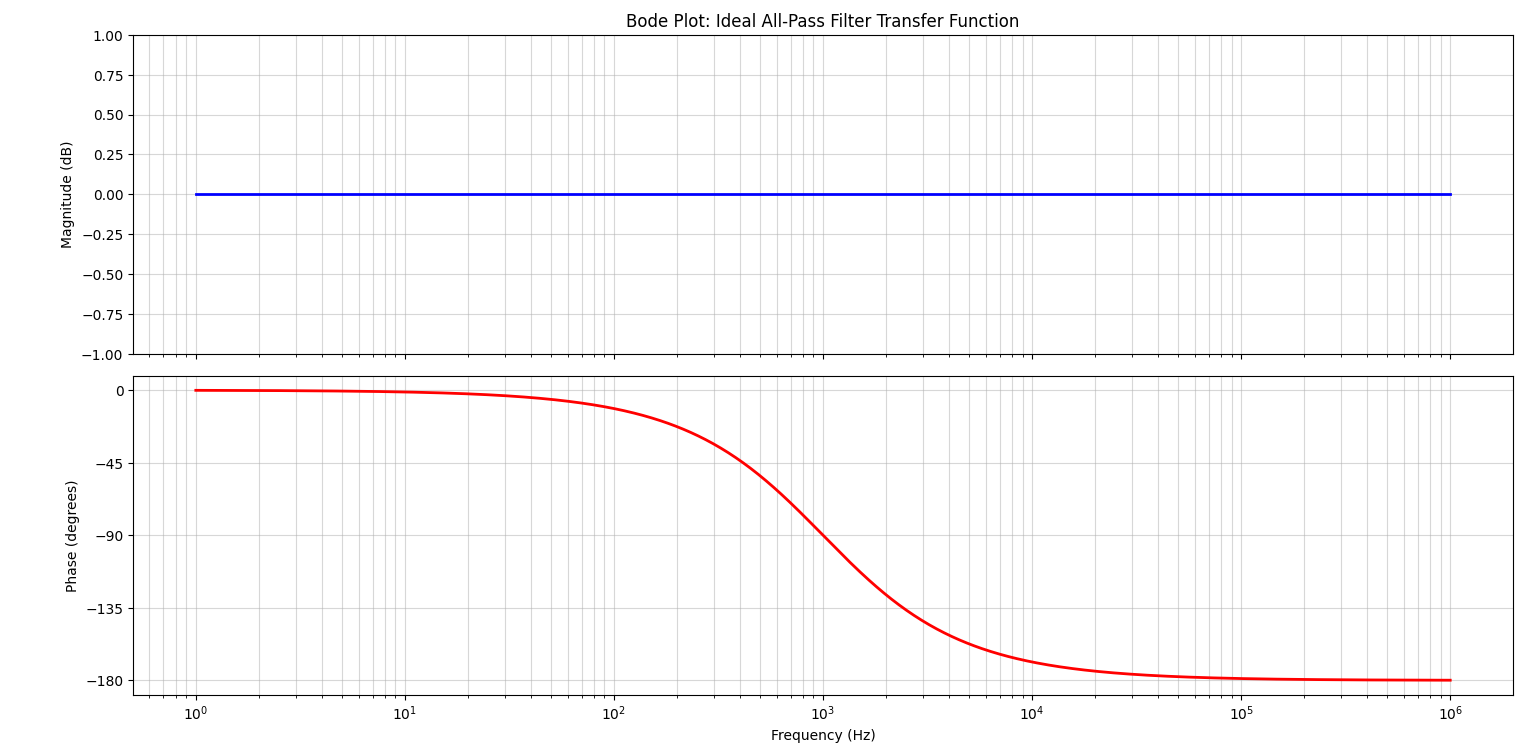
\includegraphics[width=\linewidth]{plot.png}
        \caption{Python plot}
        \label{fig:placeholder}
    \end{figure}
\end{frame}
\end{document}